%%%%%%%%%%%%%%%%%%%%%%%%%%%%%%%%%%%%%%%%%%%%%%%%%%%%%%%%%%%%%%%%%%%%%%%
%%%%%%%%%%%%%%%%%%%%%%%%%%%%%%%%%%%%%%%%%%%%%%%%%%%%%%%%%%%%%%%%%%%%%%% 
%%%%%%%%%%%       								 Preamble				         	 %%%%%%%%%% 
%%%%%%%%%%%%%%%%%%%%%%%%%%%%%%%%%%%%%%%%%%%%%%%%%%%%%%%%%%%%%%%%%%%%%%% 
%%%%%%%%%%%%%%%%%%%%%%%%%%%%%%%%%%%%%%%%%%%%%%%%%%%%%%%%%%%%%%%%%%%%%%% 
\documentclass[10pt]{beamer}
\usepackage{setspace}
\usepackage{color}
\usepackage{amsmath,lmodern}
\usepackage{hyperref}
\usepackage{graphicx}
\usepackage{multirow}
\usepackage{tikz}
\usetikzlibrary{fit,shapes.misc}
\usepackage{pdflscape}
\usepackage{amsmath}
\usepackage{lscape}
\usepackage{multirow}
\usepackage{enumerate}
\usepackage{epstopdf}
\usepackage{pdfpages}
\usepackage{appendixnumberbeamer}
\usepackage{color,soul}
\usepackage{grffile}
\usepackage{float}
\usepackage{relsize}
\usepackage{tcolorbox}
\newcounter{nodemarkers}
\usepackage{tikz}
\newcommand{\toplinesmall}{%
  \tikz[remember picture,overlay] {%
    \draw[blue,thick] ([yshift=-1cm, xshift=.9cm]current page.north west)
             -- ([yshift=-1cm,xshift=3.6cm]current page.north west);}}
             
\newcommand{\toplinemedium}{%
  \tikz[remember picture,overlay] {%
    \draw[blue,thick] ([yshift=-1cm, xshift=.9cm]current page.north west)
             -- ([yshift=-1cm,xshift=6.2cm]current page.north west);}}
 
 \newcommand{\toplinelarge}{%
  \tikz[remember picture,overlay] {%
    \draw[blue,thick] ([yshift=-1cm, xshift=.9cm]current page.north west)
             -- ([yshift=-1cm,xshift=8.9cm]current page.north west);}}           
             
 \newcommand{\toplinexlarge}{%
  \tikz[remember picture,overlay] {%
    \draw[blue,thick] ([yshift=-1cm, xshift=.9cm]current page.north west)
             -- ([yshift=-1cm,xshift=12cm]current page.north west);}}                       
             
\setbeamertemplate{footline}
{
  \leavevmode%
  \hbox{%
  \begin{beamercolorbox}[wd=.333333\paperwidth,ht=2.25ex,dp=1ex,center]{author in head/foot}%
    \usebeamerfont{author in head/foot}{\textcolor{blue}{ECON311}}
  \end{beamercolorbox}%
  \begin{beamercolorbox}[wd=.333333\paperwidth,ht=2.25ex,dp=1ex,center]{title in head/foot}%
    \usebeamerfont{title in head/foot}{\textcolor{blue}{Winter 2026}}
  \end{beamercolorbox}%
  \begin{beamercolorbox}[wd=.333333\paperwidth,ht=2.25ex,dp=1ex,right]{date in head/foot}%
    \usebeamerfont{date in head/foot}{\textcolor{blue}{Lecture 1 \: \: \: \: \: \: \: }
    \insertframenumber{} / \inserttotalframenumber\hspace*{2ex}} 
  \end{beamercolorbox}}%
  \vskip0pt%
}
\newtheorem{proposition}[theorem]{Proposition}

\newcommand\marktopleft[1]{%
    \tikz[overlay,remember picture] 
        \node (marker-#1-a) at (-0.2,1.2ex) {};%
}
\newcommand\markbottomright[1]{%
    \tikz[overlay,remember picture] 
        \node (marker-#1-b) at (0.16,-1ex) {};%
    \tikz[overlay,remember picture,thick,inner sep=4pt]
        \node[draw,rectangle,rounded corners, blue, fit=(marker-#1-a.center) (marker-#1-b.center)] {};%
}

\setbeamertemplate{caption}{\raggedright\insertcaption\par}
\setbeamertemplate{itemize items}[ball]
\setbeamertemplate{itemize subitem}[triangle]
\setbeamertemplate{itemize subsubitem}[triangle]
\tcbset{colframe=white,colback=white,nobeforeafter}
\beamertemplatenavigationsymbolsempty
\addtobeamertemplate{frametitle}{\vspace*{0.19cm}}{\vspace*{0cm}}


%%%%%%%%%%%%%%%%%%%%%%%%%%%%%%%%%%%%%%%%%%%%%%%%%%%%%%%%%%%%%%%%%%%%%%%
%%%%%%%%%%%%%%%%%%%%%%%%%%%%%%%%%%%%%%%%%%%%%%%%%%%%%%%%%%%%%%%%%%%%%%% 
%%%%%%%%%  									    Define Title									%%%%%%%%%
%%%%%%%%%%%%%%%%%%%%%%%%%%%%%%%%%%%%%%%%%%%%%%%%%%%%%%%%%%%%%%%%%%%%%%%
%%%%%%%%%%%%%%%%%%%%%%%%%%%%%%%%%%%%%%%%%%%%%%%%%%%%%%%%%%%%%%%%%%%%%%% 
\title{ECON 311: Intermediate Macroeconomic Theory} 
\author{Lecture 1: Introduction}
\date{}
\AtBeginSection[]
{
 \begin{frame}<beamer>
 \tableofcontents[currentsection]
 \end{frame}
}
%%%%%%%%%%%%%%%%%%%%%%%%%%%%%%%%%%%%%%%%%%%%%%%%%%%%%%%%%%%%%%%%%%%%%%%
%%%%%%%%%%%%%%%%%%%%%%%%%%%%%%%%%%%%%%%%%%%%%%%%%%%%%%%%%%%%%%%%%%%%%%% 
%%%%%%%% 						     				Document								       %%%%%%%%
%%%%%%%%%%%%%%%%%%%%%%%%%%%%%%%%%%%%%%%%%%%%%%%%%%%%%%%%%%%%%%%%%%%%%%%
%%%%%%%%%%%%%%%%%%%%%%%%%%%%%%%%%%%%%%%%%%%%%%%%%%%%%%%%%%%%%%%%%%%%%%% 
\begin{document}
\setbeamercovered{transparent}

\begin{frame}
\maketitle
\end{frame}


%%%%%%%%%%%%%%%%%%%%%%%%%%%%%%%%%%%%%%%%%%%%%%%%%%%%%%%%%%%%%%%%%%%%%%%
%%%%%%%%%%%%%%%%%%%%%%%%%%%%%%%%%%%%%%%%%%%%%%%%%%%%%%%%%%%%%%%%%%%%%%% 
%%%%%%%% 				Introduction to Macroeconomic Analysis		   	%%%%%%%%
%%%%%%%%%%%%%%%%%%%%%%%%%%%%%%%%%%%%%%%%%%%%%%%%%%%%%%%%%%%%%%%%%%%%%%%
%%%%%%%%%%%%%%%%%%%%%%%%%%%%%%%%%%%%%%%%%%%%%%%%%%%%%%%%%%%%%%%%%%%%%%% 

\section{Introduction to Macroeconomic Analysis}

\begin{frame}
\frametitle{\: \: \: Definitions}
\toplinesmall
\begin{itemize}
\item \textbf{Economics} is the study of how to manage scarce resources.
\vspace{.11in}
\begin{itemize}
\item Economic agents decide how to manage their scarce resources:
\vspace{.11in}
\begin{itemize}
\item E.g. workers choose how to allocate their time between labour and leisure.
\vspace{.11in}
\item E.g. consumers choose how to allocate their income across different goods and services.
\vspace{.11in}
\item E.g. firms make production decisions.
\end{itemize}
\end{itemize}
\vspace{.11in}
\item \textbf{Macroeconomics} studies the interaction of the decisions of economic agents at the national level.
\end{itemize}
\end{frame}

\begin{frame}
\frametitle{\: \: \: Definitions}
\toplinesmall
\centering
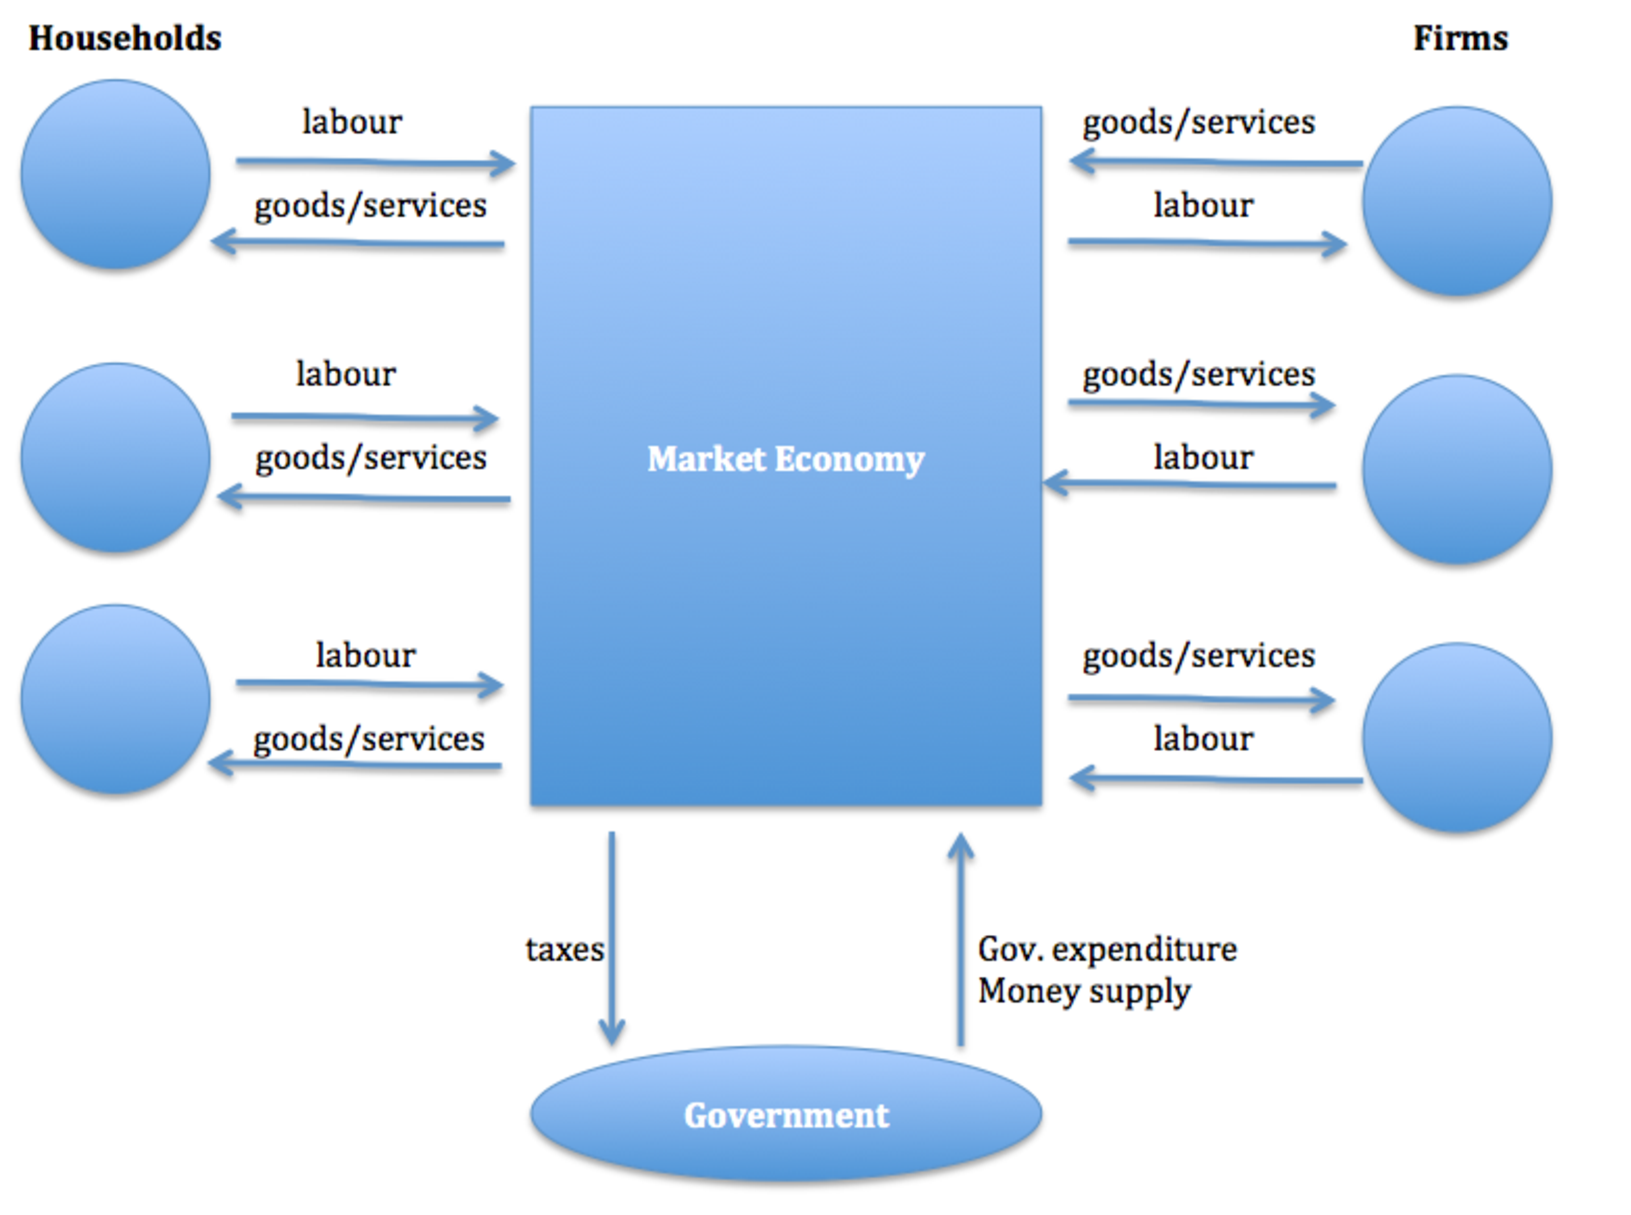
\includegraphics[scale=.34]{Market_economy}
\end{frame}

\begin{frame}
\frametitle{\: \: \: Macroeconomic Approach}
\toplinelarge
\begin{enumerate}
\item Document a set of empirical regularities or stylized facts about economies.
\vspace{.11in}
\item Develop a model that focus on relevant economic relations.  
\vspace{.11in}
\item Use data to determine the model's parameters and exogenous variables
\vspace{.11in}
\item Measure how well the model explain endogenous variables given parameters and exogenous variables.
\end{enumerate}
\end{frame}

%%%%%%%%%%%%%%%%%%%%%%%%%%%%%%%%%%%%%%%%%%%%%%%%%%%%%%%%%%%%%%%%%%%%%%%
%%%%%%%%%%%%%%%%%%%%%%%%%%%%%%%%%%%%%%%%%%%%%%%%%%%%%%%%%%%%%%%%%%%%%%% 
%%%%%%%% 				Measuring Aggregate Economic Activity		    	 %%%%%%%%
%%%%%%%%%%%%%%%%%%%%%%%%%%%%%%%%%%%%%%%%%%%%%%%%%%%%%%%%%%%%%%%%%%%%%%%
%%%%%%%%%%%%%%%%%%%%%%%%%%%%%%%%%%%%%%%%%%%%%%%%%%%%%%%%%%%%%%%%%%%%%%% 
\section{Measuring Aggregate Economic Activity}



\begin{frame}
\frametitle{\: \: \: GDP across countries}
\toplinelarge
\begin{figure}
\centering
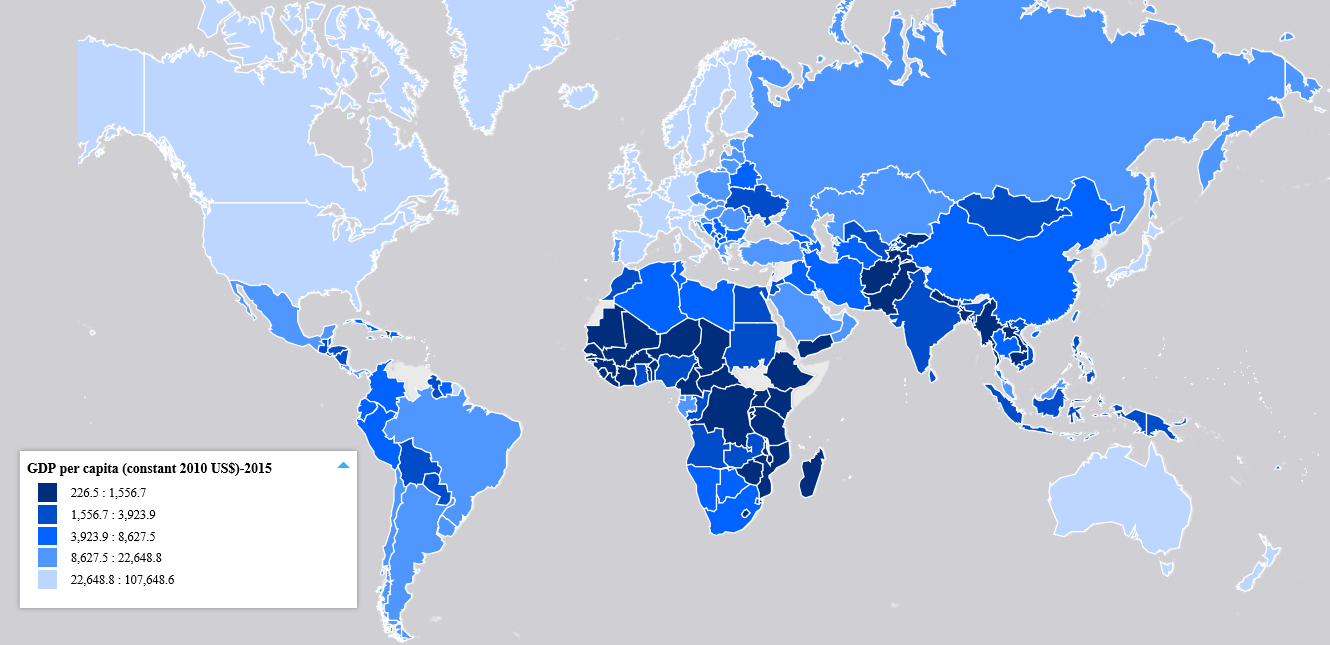
\includegraphics[scale=.4]{GDP_world}
\caption{Source: World Development Indicators}
\end{figure}
\end{frame}

\begin{frame}
\frametitle{\: \: \: GDP across countries}
\toplinelarge
\begin{figure}
\centering
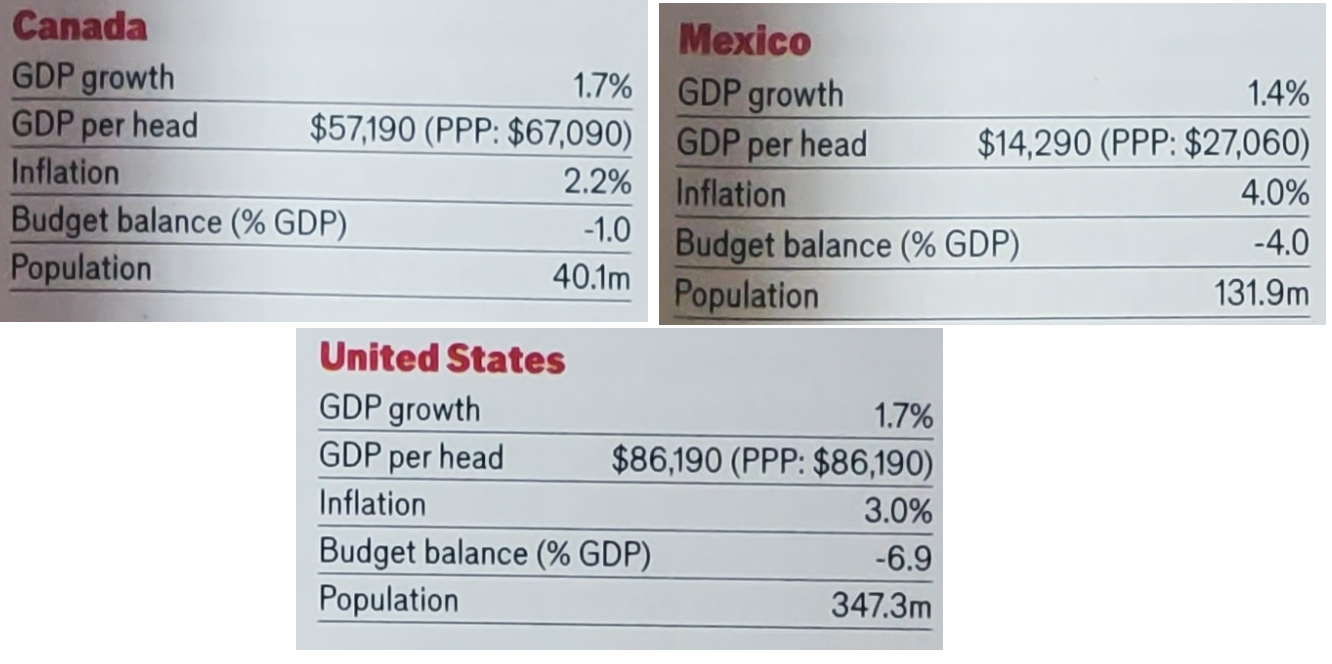
\includegraphics[scale=.4]{economist.png}
\caption{Source: The Economist}
\end{figure}
\end{frame}

\begin{frame}
\frametitle{\: \: \: GDP across time and countries}
\toplinelarge
\begin{figure}
\centering
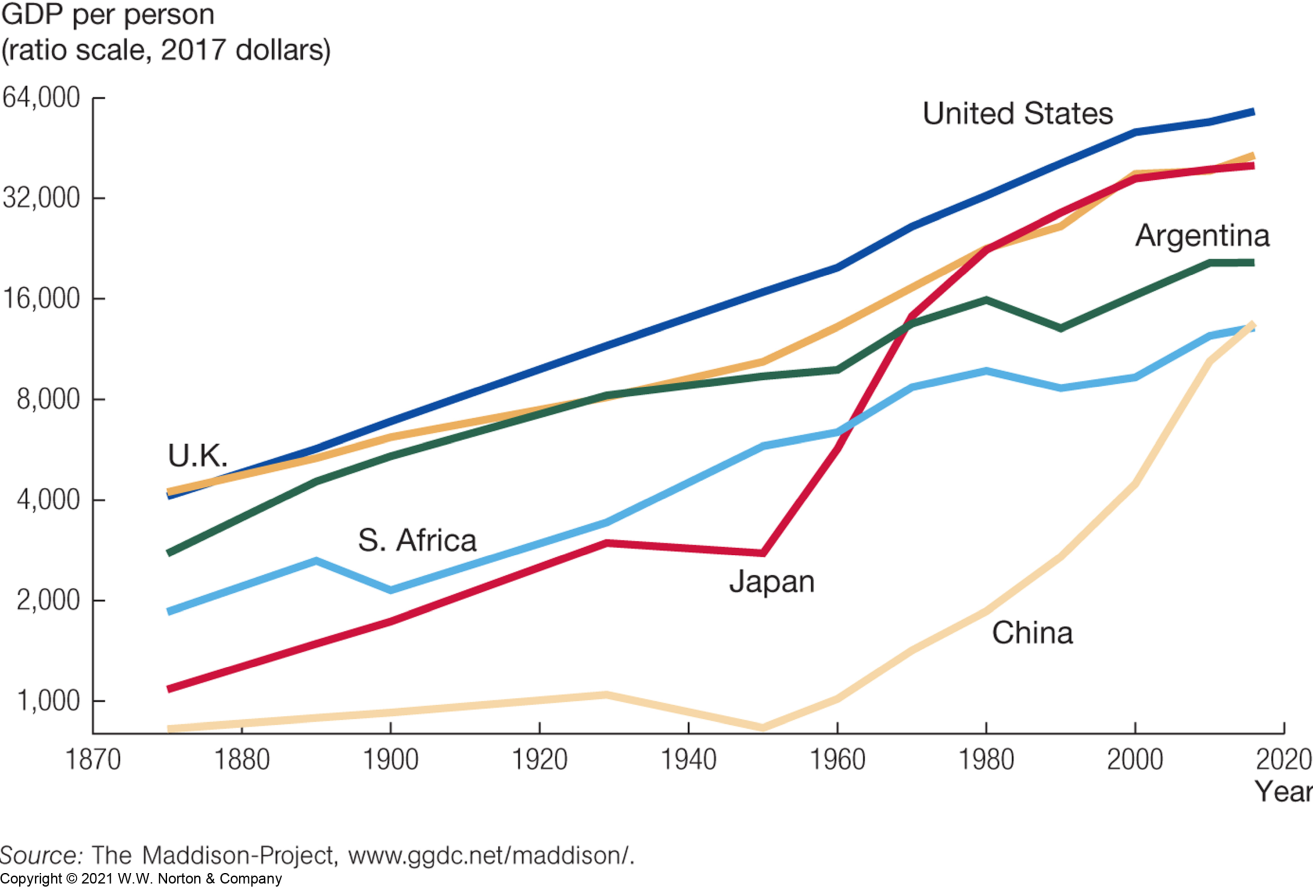
\includegraphics[scale=.37]{GDP_country_world}
\caption{Source: Macroeconomics, Jones 4E}
\end{figure}
\end{frame}

\begin{frame}
\frametitle{\: \: \: Measuring Aggregate Economic Activity}
\toplinexlarge
In \textbf{lecture 2}, we will review how economists measure aggregate economy activity.
\begin{itemize} 
\vspace{.11in}
\item In particular, we will review ...
\begin{enumerate}
\vspace{.11in}
\item different approaches to measure the value of output (ECON 101-Review)
\vspace{.11in}
\item how to compare economic activity across time (price indexes):
\vspace{.11in}
\begin{itemize}
\item Chain-Weighting Approach to measure changes in real GDP over the long-run
\end{itemize}
\vspace{.11in}
\item how to compare economic activity across countries:
\vspace{.11in}
\begin{itemize}
\item using PPP-exchange rates
\end{itemize}
\end{enumerate}
\end{itemize}
\end{frame}

%%%%%%%%%%%%%%%%%%%%%%%%%%%%%%%%%%%%%%%%%%%%%%%%%%%%%%%%%%%%%%%%%%%%%%%
%%%%%%%%%%%%%%%%%%%%%%%%%%%%%%%%%%%%%%%%%%%%%%%%%%%%%%%%%%%%%%%%%%%%%%% 
%%%%%%%% 				           Long vs Short Run		             	 %%%%%%%%
%%%%%%%%%%%%%%%%%%%%%%%%%%%%%%%%%%%%%%%%%%%%%%%%%%%%%%%%%%%%%%%%%%%%%%%
%%%%%%%%%%%%%%%%%%%%%%%%%%%%%%%%%%%%%%%%%%%%%%%%%%%%%%%%%%%%%%%%%%%%%%% 
\section{Long Run}

\begin{frame}
\frametitle{\: \: \:  Real GDP per Capita}
\toplinelarge
\begin{figure}[H]
\centering
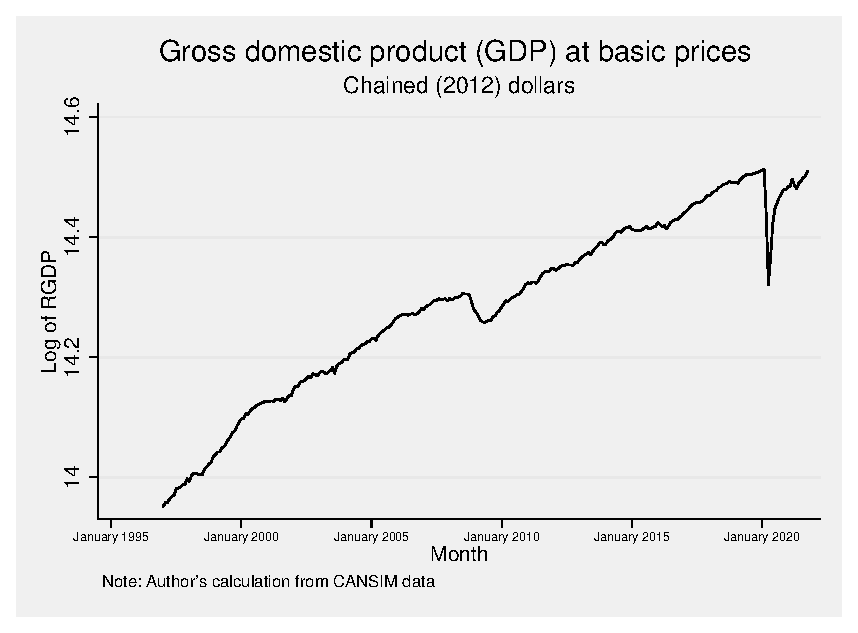
\includegraphics[scale=.65]{Canada_GDP}
\end{figure}
\end{frame}

\begin{frame}
\frametitle{\: \: \: Decomposing Real GDP per Capita}
\toplinelarge
\begin{itemize}
\item Annual average growth of real GDP per capita $1960$--$2017$$\approx$ $2.01\%$
\vspace{.11in}
\item The series is composed of a trend ($t$) and cyclical ($c$) components:
\begin{eqnarray*}
y_t=c_t+t_t 
\end{eqnarray*}
\begin{itemize}
\item \textcolor{red}{Trend component:} Underlying structure of the series  
\vspace{.11in}
\item \textcolor{red}{Cyclical component:} Temporary shocks
\end{itemize}
\end{itemize}
\end{frame}


\begin{frame}
\frametitle{\: \: \: Real GDP per Capita -- Trend}
\toplinelarge
\begin{figure}[H]
\centering
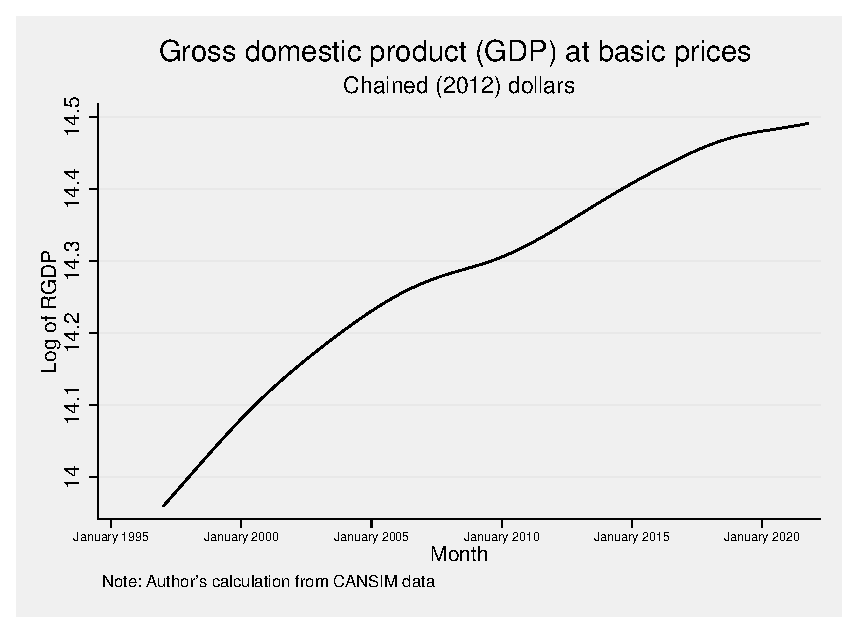
\includegraphics[scale=.65]{Canada_GDP_trend}
\end{figure}
\end{frame}

\begin{frame}
\frametitle{\: \: \: Real GDP per Capita Across Time and Countries}
\toplinexlarge
\toplinelarge
\begin{figure}[H]
\centering
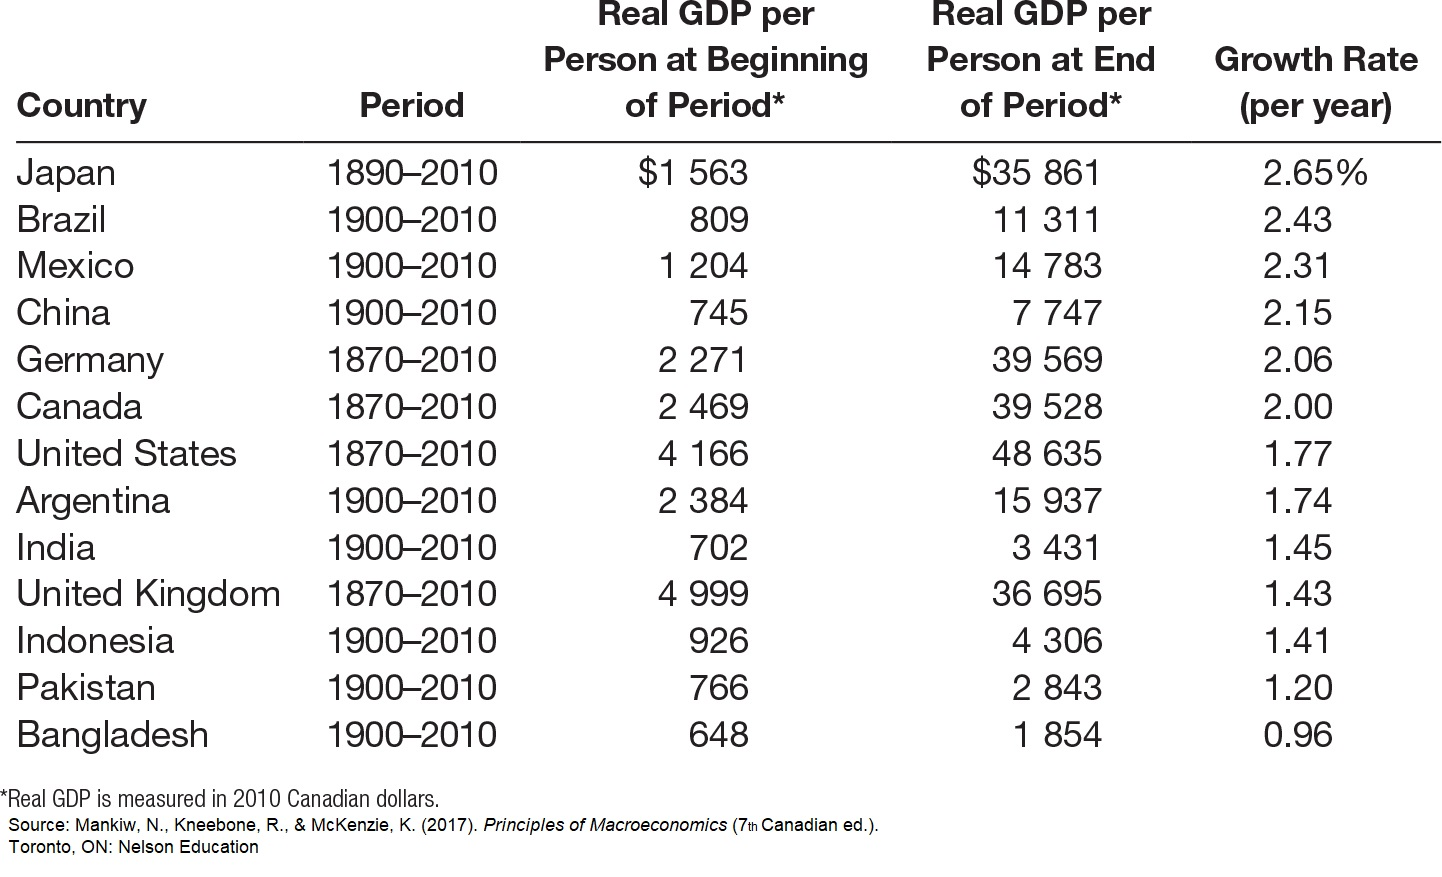
\includegraphics[scale=.85]{diff_GDP.jpg}
\end{figure}
\end{frame}

\begin{frame}
\frametitle{\: \: \: Real GDP per Capita Across Time and Countries}
\toplinexlarge
\toplinelarge
\begin{figure}[H]
\centering
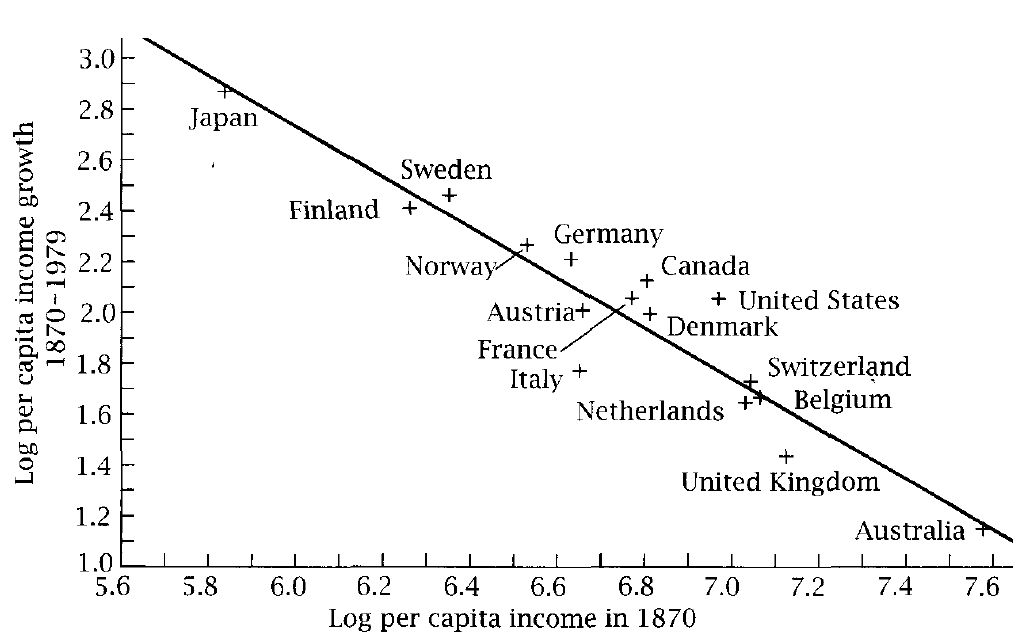
\includegraphics[scale=.45]{convergence}
\end{figure}
\end{frame}


\begin{frame}
\frametitle{\: \: \: Real GDP per Capita Across Time and Countries}
\toplinexlarge
\toplinelarge
\begin{figure}[H]
\centering
\includegraphics[scale=.55]{inequal_growth.jpg}
\caption{Notes: The ratio refers to the average of the richest 5 percent of countries to the poorest 5 percent of countries in each year. Since the sample contains 101countries, these are averages of 5 countries. Source: Restuccia 2011}
\end{figure}
\end{frame}

\begin{frame}
\frametitle{\: \: \: Long-Run Economic Growth}
\toplinelarge
\textbf{Lucas (1988): ``Once one starts to think about economic growth, it is hard to think about anything else''}
\begin{itemize}
\vspace{.11in}
\item In \textbf{lectures 3-10}, we study the determinants of long-run growth:
\begin{enumerate}
\vspace{.11in}
\item Basic facts about long-run growth across countries
\vspace{.11in}
\item Disaggregate cross-country differences in output per-capita into differences in resources to produce (growth accounting)
\vspace{.11in}
\item Study two important long-run growth model with very different implications for long-run growth:
\begin{itemize}
\vspace{.11in}
\item Solow Growth Model
\vspace{.11in}
\item Romer Growth Model   
\end{itemize}
\end{enumerate}
\end{itemize}
\end{frame}

\begin{frame}
\frametitle{\: \: \: Money and Inflation}
\toplinemedium
\begin{figure}
\centering
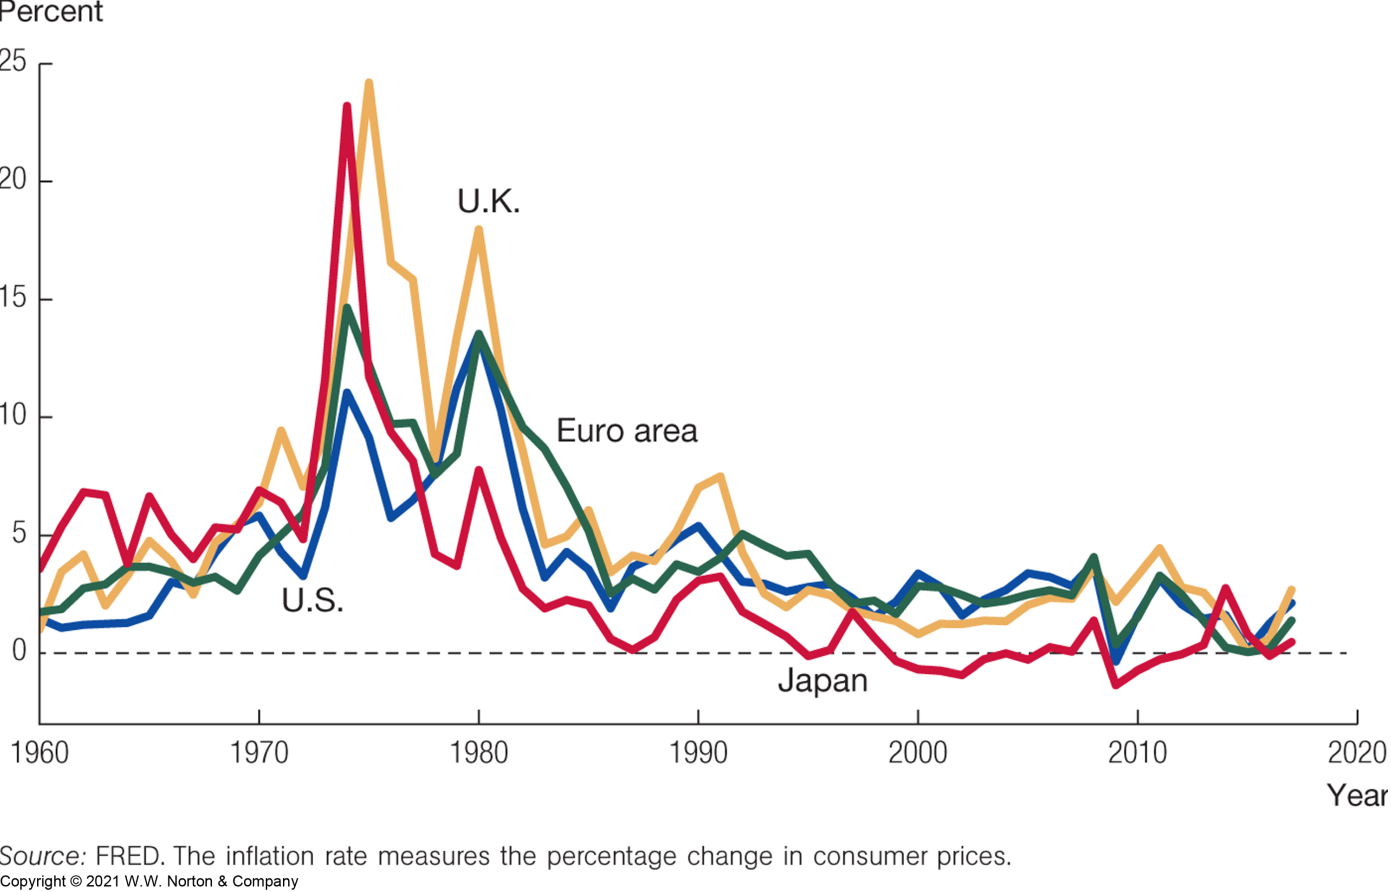
\includegraphics[scale=.37]{inflation}
\caption{Source: Macroeconomics, Jones 4E}
\end{figure}
\end{frame}

\begin{frame}
\frametitle{\: \: \: Money and Inflation}
\toplinemedium
\begin{figure}
\centering
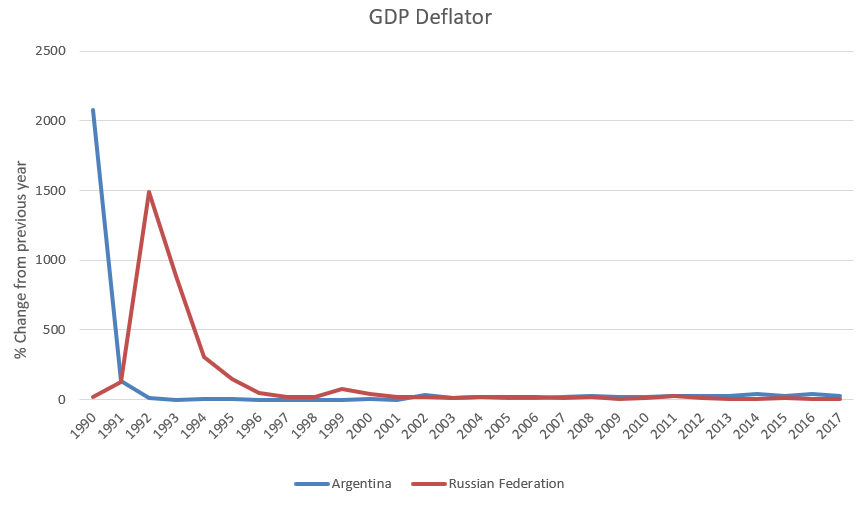
\includegraphics[scale=.55]{hyperinflation1}
\caption{Source: World Development Indicators}
\end{figure}
\end{frame}

\begin{frame}
\frametitle{\: \: \: Money and Inflation}
\toplinemedium
\begin{figure}
\centering
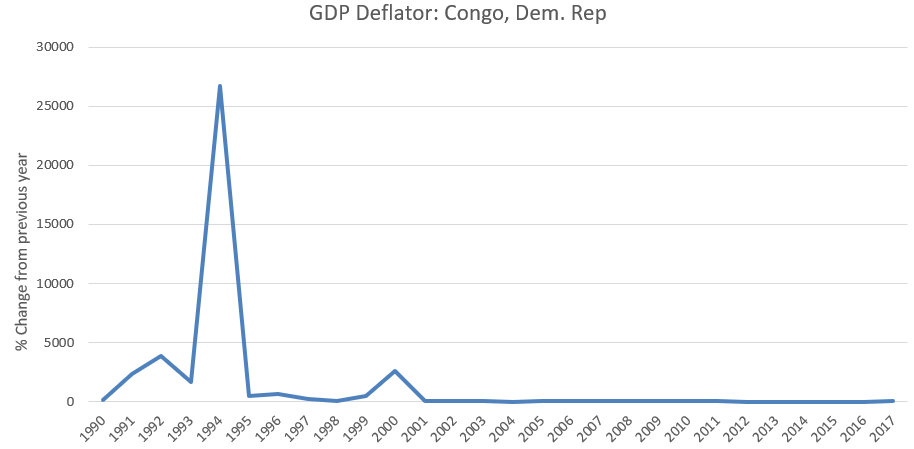
\includegraphics[scale=.55]{hyperinflation2}
\caption{Source: World Development Indicators}
\end{figure}
\end{frame}

\begin{frame}
\frametitle{\: \: \: Money and Inflation}
\toplinelarge
\begin{itemize}
\vspace{.11in}
\item In \textbf{lecture 13}, we briefly discuss the topic of inflation in the long-run:
\begin{enumerate}
\vspace{.11in}
\item Determinants of long-run inflation
\vspace{.11in}
\item The Quantity Theory of Money (relationship between the growth of money and inflation) 
\end{enumerate}
\end{itemize}
\end{frame}

\section{Short Run}

\begin{frame}
\frametitle{\: \: \: Real GDP per Capita -- Cyclical Component}
\toplinexlarge
\begin{figure}[H]
\centering
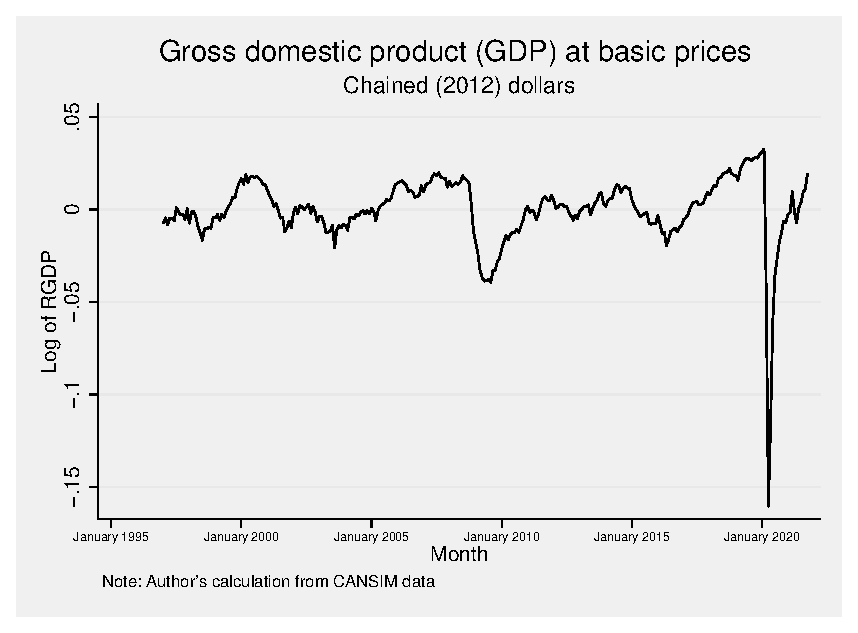
\includegraphics[scale=.65]{Canada_GDP_cycle}
\end{figure}
\end{frame}

\begin{frame}
\frametitle{\: \: \: Short-Run Economic Fluctuations}
\toplinelarge
\begin{itemize}
\vspace{.11in}
\item In \textbf{lectures 13-21}, we study the determinants of short-run economic fluctuations:
\begin{enumerate}
\vspace{.11in}
\item Basic facts about short-run deviations from potential output
\vspace{.11in}
\item Shocks to the economy, inflation and government short-run economic policy
\vspace{.11in}
\item The central macroeconomics model of short-run economic fluctuations (AS-AD model)
\end{enumerate}
\end{itemize}  
\end{frame}

\begin{frame}
\frametitle{\: \: \: Recent Economic Crisis}
\toplinelarge
\begin{itemize}
\item In our last two lectures (22 and 23), we turn our attention to studying different dimensions of the two most recent economic crisis
\begin{itemize}
\vspace{.11in}
\item The Great Recession of 2008 
\begin{figure}
\centering
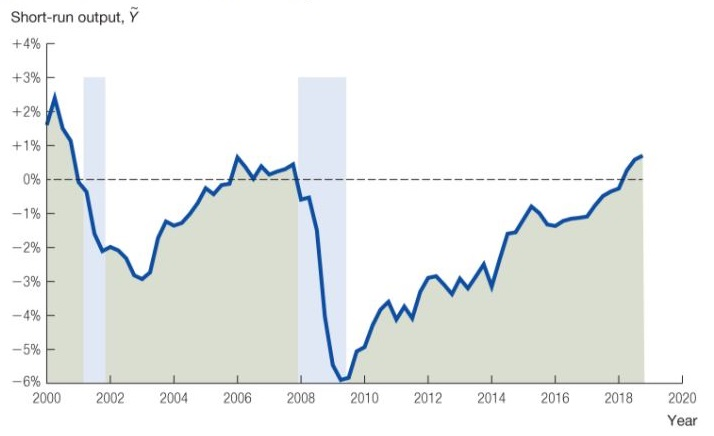
\includegraphics[scale=.55]{great_recession}
\caption{Source: Macroeconomics, Jones 4E}
\end{figure}
\end{itemize}
\end{itemize}
\end{frame}

\begin{frame}
\frametitle{\: \: \: Recent Economic Crisis}
\toplinelarge
\begin{itemize}
\item In our last two lectures (22 and 23), we turn our attention to studying different dimensions of the two most recent economic crisis
\begin{itemize}
\vspace{.11in}
\item The COVID-19 Recession 
\begin{figure}
\centering
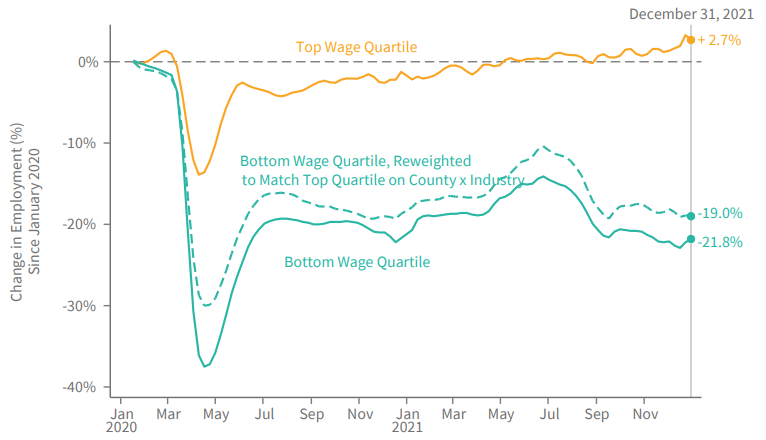
\includegraphics[scale=.42]{opportunity}
\caption{FIGURE: Changes in Employment by Wage Quartile, Source: Opportunity Insight}
\end{figure}
\end{itemize}
\end{itemize}
\end{frame}
\end{document}